\input{preamble-standalone.ltx}
\begin{document}

% Ex. No. 35 (Section  6.3.2 : Use of \tkzname{pi} and \tkzcname{tkzAxeX})

\begin{tikzpicture}
  \tkzInit[xmax=4,ymax=3.5]
  \let\tkzmathstyle\displaystyle
  \tkzLabelX[orig  = false, frac  = 4,below = 10pt]
  \tkzDrawX[label = $t$]
  \tkzAxeY[trig=2]
\end{tikzpicture}

\end{document}